%\documentclass{beamer}
\documentclass[handout]{beamer}

\usepackage{tikz,fancyvrb,hyperref,multicol,relsize,verbatim,ulem}%,enumitem}
%\usepackage{enumitem}
\usepackage{mathrsfs,mathtools,framed}
\usepackage[T1]{fontenc}


\usetikzlibrary{shapes,arrows}


%\usetheme{Warsaw}


%\usecolortheme{beaver}


\usefonttheme{professionalfonts}
%\setbeamercolor{block}{bg=red, fg=white}
\setbeamercolor{block title}{bg=blue!25}
\setbeamercolor{block body}{bg=blue!15}


\AtBeginSection[ ] {
\begin{frame}<beamer>{ }
\frametitle{Outline}
\tableofcontents[currentsection]
\end{frame} }



\newcommand{\leqAS}{\overset{\textrm{a.s.}}{\leq}}

\renewcommand{\b}{\textbf}
\newcommand{\bX}{X}
\newcommand{\bS}{\mathbf{S}}
\newcommand{\cX}{\mathcal{X}}
\newcommand{\hJ}{\widehat{J}}
\newcommand{\cI}{\mathcal{I}}
\newcommand{\cQ}{\mathcal{Q}}
\newcommand{\hcQ}{\widehat{\mathcal{Q}}}
\renewcommand{\bar}{\overline}
\newcommand{\proj}{\mathcal{P}}
\newcommand{\cY}{\mathcal{Y}}
\newcommand{\sF}{\mathscr{F}}
\newcommand{\cT}{\mathcal{T}}
\newcommand{\pow}{\textnormal{Pow}}


\newcommand{\bcol}[2]{{\usebeamercolor[fg]{#1} #2}}
\newcommand{\bstrc}[1]{\bcol{structure}{#1}}
\newcommand{\balrt}[1]{\bcol{alerted text}{#1}}

%\usepackage{multimedia}
\usepackage{../../mycommands}
\newcommand{\hk}{\hat{k}}
\newcommand{\cE}{\mathcal{E}}
\newcommand{\cN}{\mathcal{N}}
\newcommand{\Err}{\cE}

\newcommand*\mystrut{\vrule width0pt height0pt depth1.5ex\relax}
\newcommand{\underlabel}{\underbracket[1pt][.5pt]{\mystrut \quad\;\; \sub \quad\;\; }}


\title{Adaptive Sequential Model Selection}

\author{Will Fithian\\~\\
  {\small Joint with:}\\
  Jonathan Taylor,\\ Rob Tibshirani,\\ Ryan Tibshirani}
\date{\today}


\begin{document}


\frame{\titlepage}



\section{Sequential Model Selection}


\frame{\frametitle{Motivation: Model Selection in Regression}
  \bstrc{Given:} response $Y \in \R^n$, predictors $X_1,\ldots, X_p$
  \vskip+1em
  Run $d$ steps of LARS / LASSO / Forward Stepwise: 
  \vskip+1em
  $\quad\imp$ sequence of selected \bstrc{variables}
  $j_1,\ldots, j_d \in [p]=\{1,\ldots,p\}$
  \vskip+1em
  $\quad\imp$ sequence of \bstrc{active sets} 
  $E_k = j_{[k]} = \{j_1,\ldots,j_k\}$
  \[\emptyset \sub E_1 \sub \cdots \sub E_d\]
  $\quad\imp$ sequence of nested \bstrc{regression models} 
  \[
  M_0 \sub M_1 \sub \cdots \sub M_d
  \]
  \[
  M_k:\;Y \sim \cN_n(X_{E_k}\beta, \sigma^2 I_n)
  \]
  \bstrc{Goal:} choose $k$
  \vskip+1em
  \bstrc{Prior Work:} Taylor, Lockhart, Tibshirani, Tibshirani (2013); Loftus and Taylor (2014)
}

\frame{\frametitle{Motivation: Principal Components Analysis}
  \bstrc{Given:} data matrix $X \in \R^{n\times m}$, sample covariance
  \[
  S = \frac{1}{n-1} \sum_{i=1}^n (x_i - \bar x)^2
  \]
  Run $d$ steps of PCA:
  \vskip+1em
  $\quad\imp$ sequence of selected \bstrc{eigenvectors}
  $u_1, \ldots, u_d$
  \vskip+1em
  $\quad\imp$ sequence of nested \bstrc{Wishart models}
  \[
  M_0 \sub M_1 \sub \cdots \sub M_d
  \]
  \[
  M_k:\; (n-1)S \sim W_m
  \left(\lambda_0 I_m + \sum_{i=1}^k\lambda_i u_iu_i', 
    \;\;\;n-1\right)
  \]
  \bstrc{Goal:} choose $k$ 
  \vskip+1em
  \bstrc{Prior work:} Choi, Taylor, and Tibshirani (2014)
}

\frame{\frametitle{Motivation: Exploratory Model Selection}
  \bstrc{General Setup:} Data $Y\sim F$, $F$ unknown
  \vskip+1em
  Use $Y$ to \bstrc{adaptively} generate sequence of nested models
  \[
  M_0(Y) \sub M_1(Y) \sub \cdots \sub M_d(Y)
  \]
  \bstrc{Goal 1:} for $k \in [d]$, construct $p_k(Y)$ to test 
  \[
  H_{0,k}:\; F \in M_{k-1}
  \quad \text{ vs. } \quad
  H_{1,k}:\; F \in M_k \setminus M_{k-1},
  \]
  adjusting for selection
  \vskip+1em
  \bstrc{Goal 2:} choose smallest adequate model $M_{k_0}$
}

\frame{\frametitle{Which Null?}
  Regression case: Should we test \bstrc{selected model} null
  \[
  H_{0,k}:\; F\in M_{k-1} \iff 
  Y \sim \cN(X_{E_{k-1}}\beta, \;\;\sigma^2I_n)
  \]
  or \bstrc{full model} null
  \[
  \widetilde H_{0,k}:\; Y \sim 
  \cN(X_{[p]\setminus j_k}\beta, \;\;\sigma^2I_n)
  \]
  Suppose $X_1$ signal, $X_2,\ldots,X_p$ noise, $X_1$ selected at step $k=4$
  \vskip+1em
  We take \bstrc{model-centric} point of view: \\
  models $M_1,\ldots,M_3$ are incorrect
  $\imp$ want to select $M_{4}$
  \vskip+1em
  Contrast with \bstrc{variable-centric} point of view 
  (e.g., knockoffs):\\ 
  variables $j_1,\ldots,j_3$ are false discoveries
  \vskip+1em 
  Will revisit this question later...
}

\frame{\frametitle{Outline}
  \begin{enumerate}
  \item Inference for single step
    \begin{itemize}
    \item Selective $p$-values
    \item Why selected model $\gg$ saturated model
    \end{itemize}
  \item Inference for full path
    \begin{itemize}
    \item Stopping rules based on $(p_1,\ldots,p_d)$
    \item When are the $p_k$ independent?
    \end{itemize}
  \item Simulation
  \end{enumerate}
  \vspa
  Focus: \bstrc{regression} models ($\sigma^2$ known or unknown)
  \note{sigma^2 known or unknown}
}


\section{Inference for One Step}


\frame{\frametitle{Inference for Step $k$}
  At step $k$, construct valid $p_k(Y)$ to test
  \[
  H_{0,k}:\; F \in M_{k-1}(Y)
  \quad \text{ vs. } \quad
  H_{1,k}:\; F \in M_\infty(Y) \setminus M_{k-1}(Y),
  \]
  \bstrc{Selective $p$-value} for fixed model $M$
  \[
  \P_F(p_{k,M} \leq \alpha \mid M_{k-1}=M) 
  \leq \alpha, \quad \forall F \in M
  \]
  Combine to get $p_k(y) = p_{k, M}(y)$:
  \[
  \P_F\left(p_k \leq \alpha \mid M_{k-1}\;F\in M_{k-1}\right) 
  \leqAS \alpha
  \]
  \note{F not random, but the models and $p$-values are}
  How to get $p_{k,M}$?
}

\frame{\frametitle{Fixed-Question Analysis}
  Must condition on \bstrc{selection event}:
  \[
  A_M=\{M_{k-1}(Y) = M\}
  \]
  $A_M$ depends on selection rule
  \vskip+1em
  Regression: $A$ is typically union of polytopes
  \vskip+1em
  
}

\frame{\frametitle{Why Condition on $M_{k-1}$?}
  What about controlling
  \[
  \P_F(p_k \leq \alpha \mid F\in M_{k-1})
  \leq \alpha
  \]
  Do we need to condition on $M_{k-1}$?
  \vskip+1em
  Could be very \bstrc{anti-conservative} for some $M$,
  and conservative for others: would that be OK?
}

\frame{\frametitle{Regression Models}
  At step $k$ add variable $j_k$, active set $E_k = \{j_1,\ldots,j_k\}$
  \vskip+1em
  Regression models for active set $E$, variable $j\in E$:
  \begin{itemize}
  \item \bstrc{Selected model:} test $H_0:\;\beta_j = 0$ in
    \[
    M:\; Y \sim \cN(X_E\beta, \;\sigma^2I), \quad (\sigma^2 \text{ kn.       / unkn.})
    \]
  \item \bstrc{Saturated model:} test $H_0:\;\eta_{j,E}'\mu = 0$ in 
    \[
    M:\; Y \sim \cN(\mu, \;\sigma^2I), \qquad (\sigma^2 \text{ known})\qquad
    \]
  \item \bstrc{Full model:} test $H_0:\; \beta=0$ in
    \[
    M:\; Y \sim \cN(X\beta, \;\sigma^2I), \quad (\sigma^2 \text{ kn. / unkn.})
    \]
  \end{itemize}
  \note{null hypotheses nested only in selected model, 
    otherwise just seq. of hyp in the same model. However,
    saturated model tests are valid for the selected model null,
    so we do have the option.}
}

\frame{\frametitle{Selected-Model Analysis}
  Selected model for active set $E_k$:
  \[
  M_k:\;Y\mid A \sim \exp\left\{\frac{1}{\sigma^2} y'X_{E_k}\beta
    - \frac{1}{2\sigma^2}\|y\|^2 - \psi_A(\beta,\sigma^2)\right\}\; 1\{y \in A\}
  \]
%  Let $T_k$ denote suff. stats for $M_k$:
%  \[
%  T_k(y) = \left(X_{E_k}'y, \|y\|^2\right) \quad \text{ if } \sigma^2 \text{unkn.}
%  \]
%  Test is based on 
  Condition on $X_{E_{k-1}}'Y$ $\rightarrow$ tests based on
  \[
  \L_{\beta_j=0}\left( X_{j_k}'Y \mid Y\in A,\;X_{E_{k-1}}'Y, \; \balrt{\|Y\| ?}\right)
  \]
  Note:
  \begin{itemize}
  \item $M_k$ has one more suff stat than $M_{k-1}$
    \note{so we add one ss to model and then test whether it helps}
  \item $p_{k,M}$ function of suff stats of $m_k$
    \note{not true for saturated model}
  \item $p_{k,M}$ conditions on suff stats of $m_{k-1}$
  \end{itemize}
}

\frame{\frametitle{Selected Model vs Saturated Model}
  \bstrc{Simple setting:} $n = p = 2, X = I_2, \sigma^2=1$ known
  \vskip+1em
  $\mu = \binom{4}{4}$. First step of forward stepwise:
  \vspa
  \begin{center}
  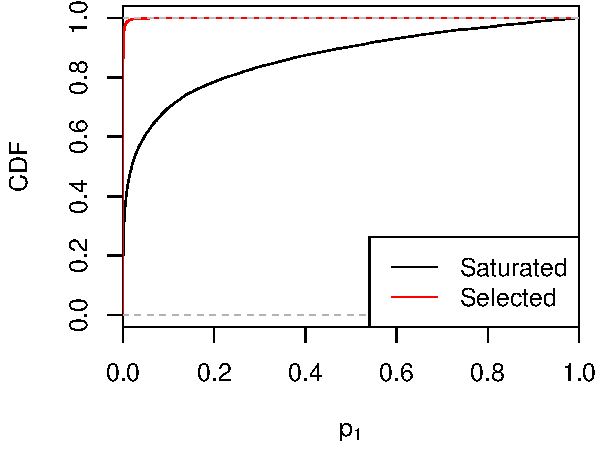
\includegraphics[width=.7\textwidth]{../../figs/bivariateSelVSat_rocCurve.pdf}
  \end{center}
  \bstrc{Power:} 99.7\% vs. 59\% for $\alpha=.05$
}

\frame{\frametitle{Selected Model vs Saturated Model}
  \bstrc{Sel.:} $Y \sim \cN\left(\binom{\mu_1}{0}, \;I_2\right)$
  $\rightarrow$ compare to $\L_{\mu=0}(Y_1 \mid A)$
  \vskip+1em
  \bstrc{Sat.:} $Y \sim \cN\left(\binom{\mu_1}{\mu_2}, \;I_2\right)$
  $\rightarrow$ compare to $\L_{\mu_1=0}(Y_1 \mid Y_2, \;A)$
  \vspa
  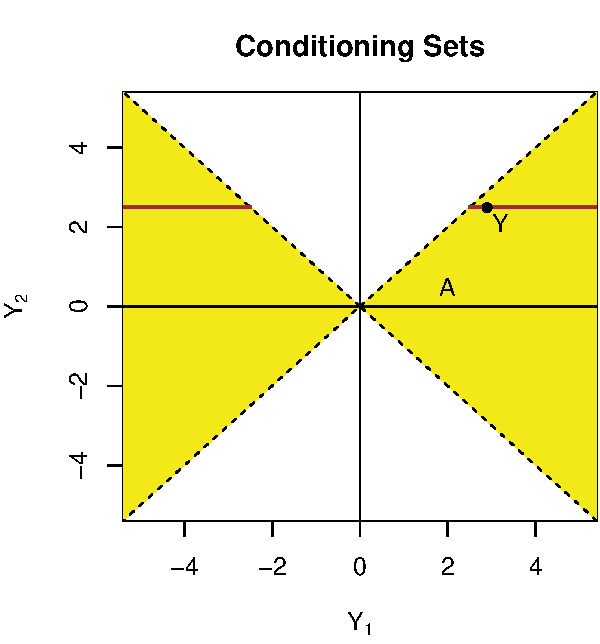
\includegraphics[width=.46\textwidth]{../../figs/bivariateSelVSat_condSets.pdf}
  \hspace{.03\textwidth}
  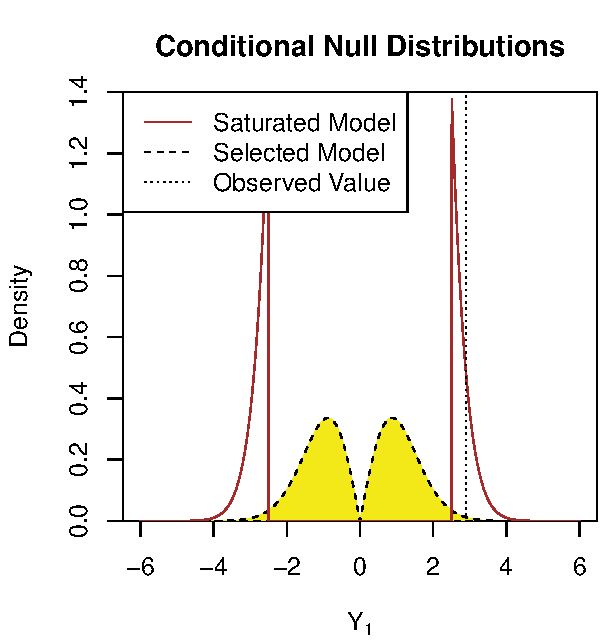
\includegraphics[width=.46\textwidth]{../../figs/bivariateSelVSat_nullDists.pdf}
}


\section{Sequential Hypothesis Testing}


\frame{\frametitle{Stopping Rules}
  Observe $Y \sim F$
  \vskip+1em
  Given \bstrc{adaptive} sequence of nested statistical models
  \[
  M_0(Y) \sub M_1(Y) \sub \cdots \sub M_d(Y) 
  \]
  and $p$-values $p_{[d]}(Y)$
  \note{stochastically smaller}
  \vskip+1em
  \bstrc{Completion index:} $k_0(Y) = \min \{k:\; F \in M_k\}$ \pause
  (first correct model)
  \vskip+1em
  \bstrc{Stopping rule:} $\hk(Y)$ estimator of $k_0$.
  \vspa
  \bstrc{Goal 2a:} Control type I errors  $(\hk - k_0)_+$
  \vskip+1em
  \bstrc{Goal 2b:} Minimize type II errors $(k_0 - \hk)_+$
}

\frame{\frametitle{Simple Stop}
  ``Obvious'' rule: stop first time $p_k > \alpha$
  \[
  \hk_{\text{simple}}(Y) = \min\left\{k \in \{1,\ldots,m\} :\;
    p_k > \alpha\right\} - 1
  \]
  For fixed $k_0$, controls \bstrc{familywise error rate:}
  \[
  \P\left[\hk_{\text{simple}}(Y) > k_0\right] \leq \alpha
  \]
  Proof:
  \begin{align*}
  \P\left[\hk_{\text{simple}} > k \right] 
  &= \P[p_{k_0+1} \leq \alpha] \\
  &\leq \alpha 
  \end{align*}
  \pause
  Random $k_0$: need $p_k$ valid given $k_0 = k-1$\\
  \vskip+1em
  \quad ($F\in M_{k-1} \iff k_0 \;\balrt{\leq}\; k-1$)
}

\frame{\frametitle{Strong Stop}
  G'Sell, Wager, Chouldechova, \& Tibshirani (2013):
  \[
  \hk_{S}(Y) = \max\left\{k \in \{1,\ldots,d\} :\;
    \exp\left(\sum_{i=k}^d \frac{\log p_i}{i}\right) 
    \leq \frac{\alpha k}{d}\right\}
  \]
  Controls \bstrc{familywise error rate:}
  \[
  \P\left[\hk_S(Y) > k_0\right] \leq \alpha
  \]
  for fixed $k_0$, under independence condition:
  \[
  (p_{k_0+1},\ldots,p_d) \mid (p_1, \ldots, p_{k_0}) 
  \sim \text{Unif}[0,1]^{d-k_0}
  \]
}

\frame{\frametitle{Forward Stop}
  G'Sell, Wager, Chouldechova, \& Tibshirani (2013):
  \[
  \hk_{F}(Y) = \max\left\{k \in \{1,\ldots,d\} :\;
    -\frac{1}{k}\sum_{i=1}^k \log(1-p_i) \leq \alpha\right\}
  \]
  Controls \bstrc{false discovery rate:}
  \[
  \E\left[\frac{(\hk_F(Y) - k_0)_+}{\hk_F(Y) \vee 1}\right] \leq \alpha
  \]
  for fixed $k_0$, under independence condition:
  \[
  (p_{k_0+1},\ldots,p_d) \mid (p_1, \ldots, p_{k_0}) 
  \sim \text{Unif}[0,1]^{d-k_0}
  \]
}

\frame{\frametitle{Pathwise $p$-Values}
  What do we need for \balrt{random} $k_0$?
  \vskip+1em
  \bstrc{Simple Stop:} need
  \[
  \P(p_k \leq \alpha \mid k_0=k) \leqAS \alpha
  \]
  \bstrc{Strong \& Forward Stop:} need
  \[
  \P\left(p_{k+1}\leq \alpha_{k+1}, \ldots, 
    p_d \leq \alpha_d
    \mid p_{[k]},\; k_0(Y)=k\right) 
  \leqAS \prod_{i=k+1}^d \alpha_i
  \]
  \bstrc{Single-Step:} before, we had
  \[
  \P_F\left(p_k \leq \alpha \mid M_{k-1},\; M_k,\; F\in M_{k-1}\right)
  \leqAS \alpha
  \]
  \balrt{Not sufficient!} \pause What would be?
  \note{so what more do we need to condition on at stage $k$ to get 
    the kind of pathwise properties we want?}
}

\frame{\frametitle{Pathwise $p$-Values}
  For filtration
  \[
  \sF_0 \sub \sF_1 \sub \cdots \sub \sF_d,
  \]
  with $M_k\sub M_{\infty}$, meas. wrt $\sF_k$ for $k=1,\ldots,d$\\
  \quad \balrt{NB:} $M_k$ random, not $F$
  \vskip+1em
  $p_{[k]}$ \bstrc{pathwise $p$-values} for hypotheses 
  $H_k:\; F\in M_{k-1}$ if
  \begin{itemize}
  \item $p_k$ conservative given $\sF_{k-1}$, for $F\in M_{k-1}$
  \item $p_k$ meas. wrt $\sF_k$
  \end{itemize}
}

\frame{\frametitle{Pathwise $p$-Values}
  For pathwise $p_k$, $F\in M_\infty$,
  \[
  \P_F\left(p_{k+1} \leq \alpha_{k+1}, \ldots,  p_d \leq \alpha_d\;\; 
    \mid k_0\leq k, \; \sF_k\right) \leqAS \prod_{i=k+1}^d \alpha_i
  \]
  Proof:
  \[
  \P_F\left(p_{k+1} \leq \alpha_{k+1}, \ldots,  p_d \leq \alpha_d\;\; 
    \mid k_0=k, \; \sF_k\right) 
  = \E_F\left[ 1\{p_{k+1}\leq \alpha_{k+1}\} 
    \P_F\left(p_{k+2} \leq \alpha_{k+2}, \ldots, p_d \leq alpha_d\;\; 
      \mid k_0\leq k+1, \; \sF_{k+1}\right)
    \;\;\mid\;\; \sF_k\right]
  \] 
}

\frame{\frametitle{Pathwise Filtration}
  Assume each model $M$ has sufficient statistics $T(Y;\;M)$\\
  \quad(regression: $T(Y;\; M(E)) = X_{E}'Y$)
  \vskip+1em
  Define $T_k(Y) = T(Y;\; M_k(Y))$  (e.g., $T_k(Y) = X_{E_k}'Y$)
  \vskip+1em
  Define \bstrc{pathwise filtration} 
  \[
  \sF_0 \sub \sF_1 \sub \ldots \sub \sF_d
  \]
  for $\sF_k = \sF(M_{[k]}, \; T_k(Y))$
}

\frame{\frametitle{Facts}
  \bstrc{Recall:} Before, just required that $p_k$ conservative 
  given $M_{k-1}$; how much more have we conditioned on?
  \vskip+1em
  \bstrc{Fact:} If $T_k$ complete suff. and $p_k$ exact selective,
  then $p_k \mid M_k, T_k \sim \text{Unif}[0,1]$.\\
  \quad Saturated-model, selected-model, max-T, next-$\lambda$, 
  etc. etc.
  \vskip+1em
  \bstrc{Fact:} If path algo $M_{[d]}(\cdot)$ satisfies SPSP then
  $\sF(M_{[k]}, T_k) = \sF(M_k, T_k)$.\\
  \quad LARS, Forward stepwise (\& generalizations), 
  LASSO (\& generalizations)
}

\frame{\frametitle{Pathwise $p$-Values: Examples}
  Selected model: \bstrc{yes, always}
  \vskip+1em
  Saturated model: \balrt{no, cannot repair}
  \vskip+1em
  Conditional max-T: \bstrc{yes, for forward stepwise}
}

\section{Simulation: Sparse Linear Regression}

\frame{\frametitle{Generating Model}
  Regression with $n=100, p=40$ 
  \[Y \sim N(X\beta, I_n)\]
  \vskip+1em
  True $\beta_j = \left\{\begin{matrix}5 & j = 1,\ldots,7\\ 0 &
      j>7\end{matrix}\right.$
  \vskip+1em
  % Use $\lambda = 2\E(\|X'\epsilon\|_\infty), \quad \epsilon \sim
  % N(0,I)$ (Negahban et al., 2012)
  % \vskip+1em
  $X$ correlated Gaussian, $\rho = 0.3$, normalized ($\text{SNR}=5$)
  \vskip+1em
  \bstrc{Selection:} Forward stepwise path, $k=1,\ldots,40$
}

\frame{\frametitle{Power}
  $p_k$ when $M_{k-1}$ is false: 
  Saturated, \balrt{Selected}, \bstrc{Nominal} 
  \begin{center}
    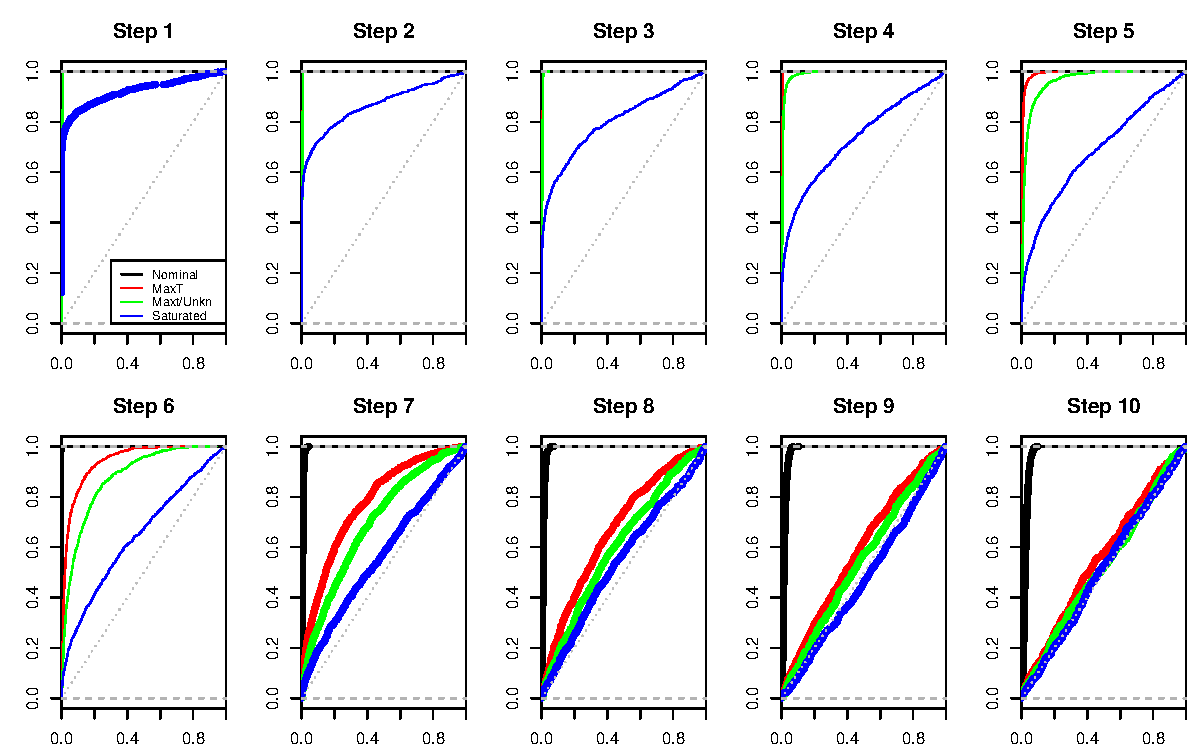
\includegraphics[width=\textwidth]{../../figs/simulation_snr_5_alpha_05_null_false.pdf}
  \end{center}
}

\frame{\frametitle{Size}
  $p_k$ when $M_{k-1}$ is true: 
  Saturated, \balrt{Selected}, \bstrc{Nominal}
  \begin{center}
    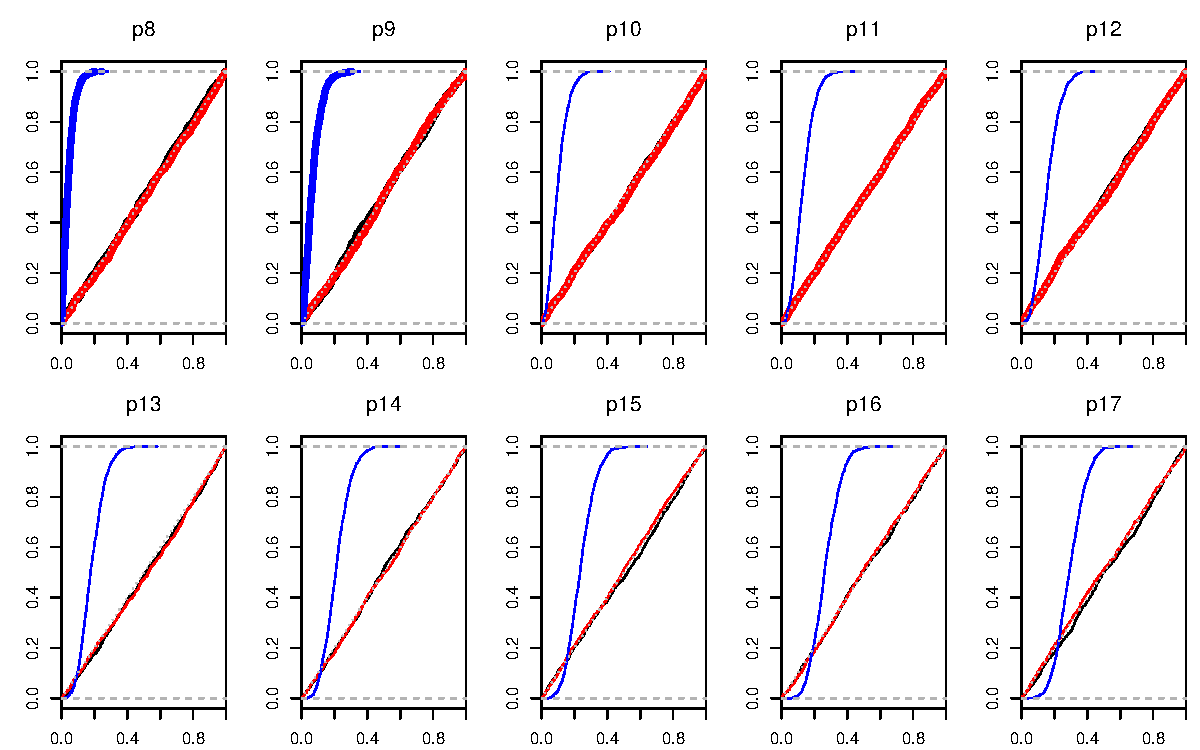
\includegraphics[width=\textwidth]{../../figs/simulation_snr_5_alpha_05_null_true.pdf}
  \end{center}
}

\frame{\frametitle{Caveat Emptor}
  $p_k$ when $j_k$ is a noise variable:
  Saturated, \balrt{Selected}, \bstrc{Nominal}
  \begin{center}
    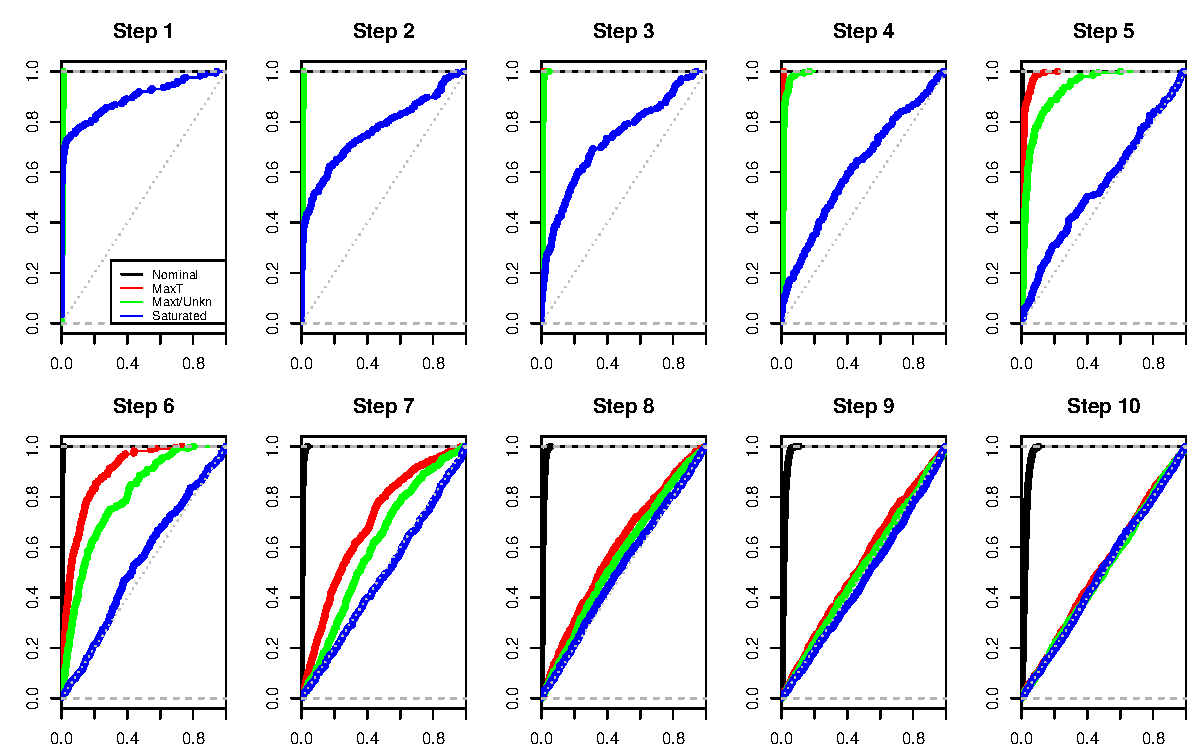
\includegraphics[width=\textwidth]{../../figs/simulation_snr_5_alpha_05_noise_var.pdf}
  \end{center}
}

\frame{\frametitle{Model Selection Performance}
  Define
  \[
  V_{\text{mod}} = (\hat k - k_0)_+, 
  \quad V_{\text{var}} =  \#\{\text{noise var.s included}\},
  \quad R = \hat k
  \]
  Then
  \[
  \text{FDR}_{*} = \E[V_{*} / (R \vee 1)], \quad
  \text{FWER}_{*} = \P[V_{*} > 0]
  \]
  % latex table generated in R 3.0.2 by xtable 1.7-1 package
  % Fri May  1 09:29:28 2015
  \begin{table}[ht]
    \centering
    \begin{tabular}{llcccc}
      \hline
      & & $p_{\text{screen}}$ & $\text{FWER}_{\text{mod}}$ 
      & $\text{FDR}_{\text{mod}}$ 
      & $\text{FDR}_{\text{var}}$ \\ 
      \hline
      Selected & Simple & .290 & .000 & .002 & .039 \\ 
      Selected & Forward & .559 & .027 & .020 & .066 \\ 
      Selected & Strong & .041 & .014 & .008 & .042 \\ 
      \hline
      Saturated & Simple & .000 & .000 & .000 & .028 \\ 
      Saturated & Forward & .014 & .000 & .000 & .030 \\ 
      Saturated & Strong & .000 & .000 & .000 & .032 \\ 
      \hline
      Knockoffs & & .000 &  &  & .231 \\ 
      \hline
    \end{tabular}
  \end{table}
}

\frame{\frametitle{Summary}
  Takeaways:
  \begin{enumerate}
  \item Selected model is more powerful than saturated model 
    when we have ``near ties''
  \item Selected-model inference automatically gives independent
    $p$-values\\
    \quad (but not saturated-model inference)
  \end{enumerate}
}

\frame{\frametitle{The End}
  \begin{center} 
    {\Huge Thanks!}
  \end{center}
}











\begin{comment}
\frame{\frametitle{Relating Single-Step to Pathwise}
  Just need to condition on $M$, $p$ up to step $k-1$
  \begin{block}{Lemma (FTTT 2015)}
    Assume that for all $F,k,\alpha$,
    \[
    \P_F\left(p_k \leq \alpha \mid M_{[k-1]}, \;p_{[k-1]}, 
      \;F \in M_{k-1}\right) \leqAS \alpha.
    \]
    Then, 
    \[
    \P_F\left(p_{k+1}\leq \alpha_{k+1}, \;\ldots, \;p_d \leq \alpha_d
      \mid p_{[k]}, \;k_0(Y)=k\right) 
    \leqAS \prod_{i=k+1}^d \alpha_i 
    \]
  \end{block}
  \vspa
  \balrt{Surprise:} selected model test (usually) gets this for free!
  %Proof:
  %\[
  %\P_F\left(p_d \leq \alpha_d \mid p_{[d-1]}, k_0(Y)=k\right) 
  %\leqAS \alpha_d
  %\]
}

\frame{\frametitle{Nested Exponential Families}
  \bstrc{Special Case:} 
  models are exponential families with nested suff. stats
  \[
  M_k:\; y \sim 
  \exp\left\{ \sum_{i=0}^k \theta_i \,T(y;\;\gamma_i)
    - \psi_{k}(\theta)\right\} f_0(y)
  \]
  New suff. stat. at step $k$ selected adaptively 
  ($\gamma_k = \gamma_k(Y)$) 
  \vspa
  \quad e.g., selected linear models with nested $E_k$
  \begin{itemize}
  \item $T_0(y) =  \|y\|^2$ \quad if $\sigma^2$ unknown
  \item $T_k(y) = X_{j_k}'y$ \quad for $k \geq 1$
  \end{itemize}
  \vspa
  \quad e.g., Wishart for nested PCA models
}

\frame{\frametitle{Assumptions}
  \bstrc{1. Assume:} given $M_k=m_k$, 
  path $M_{[k]}$ depends only on $T_{[k]}$
  \vskip+1em
  \quad \bstrc{``sub-path sufficiency principle''}
  \vskip+0.5em
  \quad \bstrc{Regression:} say, $E_3 = \{1,3,6\}$.
  \vskip+0.25em
  \qquad $\Rightarrow$ order of first 3 variables only depends 
  on $X_{\{1,3,6\}}'Y$
  \vskip+0.5em
  \quad true for forward stepwise, LARS, LASSO
  \vspa
  
  \bstrc{2. Assume:} 
  \begin{itemize}
  \item $p_{k,M}$ function of $T_{[k]}$
  \item $p_{k,M}$ uniform given $T_{[k-1]}$
  \end{itemize}
  \vskip+0.5em
  \quad true for UMPU or equal-tailed $p_k$ for \bstrc{selected model}
  \vskip+0.5em
  \quad \balrt{not} true for saturated model!
}

\frame{\frametitle{Result}
  \begin{block}{Theorem (FTTT 2015)}
    For nested exponential family models where assumptions 
    1 \& 2 hold, single-step $p$-values satisfying
    \[
    \P_F\left(p_k \leq \alpha \mid M_{k-1}, M_k, 
      \;F \in M_{k-1}\right) \leqAS \alpha
    \]
    also satisfy
    \[
    \P_F\left(p_{k+1}\leq \alpha_{k+1}, \;\ldots, \;p_d \leq \alpha_d
      \mid p_{[k]}, \;k_0(Y)=k\right) 
    \leqAS \prod_{i=k+1}^d \alpha_i 
    \]
  \end{block}
  
  \bstrc{Interpretation:} Selected model test + LASSO / LARS / Forward Stepwise + Simple / Strong / Forward Stop \balrt{works}
  
}
\end{comment}



\end{document}





